\documentclass{article}

%math stuff
\usepackage{amsmath}
\usepackage{enumitem}
\usepackage{mathtools}
\usepackage{listings}

%bibliography/appendix
\usepackage{cite}
\usepackage[toc,page]{appendix}

%figures
\usepackage{graphicx}
\usepackage{booktabs}

%General Formating
\renewcommand*\familydefault{\sfdefault}
\usepackage[letterpaper, portrait, margin=1.5in]{geometry}
\usepackage{fancyhdr}
\pagestyle{fancy}

%Header
\lhead{Schulman}
\rhead{Page \thepage}

\title{Econometrics I Homework 1}
\author{Eric Schulman}
\date{\today}

\begin{document}

\maketitle

\section{Part I}

\begin{enumerate}
	\item[2.2] 

	$$E( E(xy | x))$$
	$$ = E( xE(y | x))$$
	$$ = E(a(x+bE(x))|x)$$
	$$a(x+bE(x))$$
	
	\item[2.4]

	$$E(y|x=0) = E(y^2 |x=0)  = .8$$
	$$E(y|x=1) = E(y^2 |x=1)  = .6$$
	$$E(y^2|x=0) - (E(y|x=0))^2 = .16$$
	$$E(y^2|x=1) - (E(y|x=1))^2 = .24$$

	\item[2.5]
	\begin{enumerate} [label=\alph*)]
    	\item 

    	$$E((e^2-g(x))^2)$$
        
        \item 

        $$\text{Minimize } E((e^2-h(x))^2)$$
        
        \item 

        $$E((e^2-g(x))^2)$$
        $$ = E((e^2-\sigma^2(x) + \sigma^2(x) - h(x))^2)$$
        $$ = E((e^2-\sigma^2(x))^2) + E((\sigma^2(x) -h(x))^2) + 2E((\sigma^2(x) -h(x))(e^2-\sigma^2(x)))$$

        Since $$E((\sigma^2(x) -h(x))(e^2-\sigma^2(x)))$$
        $$ = E(E((\sigma^2(x) -h(x))(e^2-\sigma^2(x))|x))$$
        $$ = E(E(e^2\sigma^2(x) - e^2g(x) + g(x)\sigma^2(x) +\sigma^2(x) \sigma^2(x)|x))$$
        $$ = E(\sigma^2(x)\sigma^2(x) - \sigma^2(x)g(x) + g(x)\sigma^2(x) +\sigma^2(x) \sigma^2(x)) = 0$$

        We have
        $$E((e^2-g(x))^2) = E((e^2-\sigma^2(x))^2) + E((\sigma^2(x) -h(x))^2) \geq E((e^2-\sigma^2(x))^2) $$
    
    \end{enumerate} 

    \item[2.7]
    $$E(y^2|x) - (E(y|x))^2 = V(y|x) = V(\beta x + e |x) = V(e|x) = \sigma^2(x)$$

    \item[2.10] True

    $$E(x^2e) = E(x^2 E(e|x) ) = 0$$

    \item[2.11] False

    Suppose $e$ has a degenerate distribution and $p(x=1) = .5$ and $p(x=-1) = .5$

    $$E(ex) = 0$$
    $$E(ex^2) = \bar{e} $$

    \item[2.12] False.

    Suppose $e,x$ are uniformly distributed across the unit circle around $(0,0)$. The conditional distribution of $e$ given $x$ is uniform over the interval $(-\sqrt{1-x^2},\sqrt{1-x^2})$, So its expectation, found by integrating the conditional density, is zero.

    However,they share a distribution so they are not independent.


    $$E(e|x) = 0$$

    \item[2.13] Use the same counter example as 2.11

    $$E(ex) = 0$$
    $$E(e|x) = \bar{e} $$


    \item[2.14] False

    Suppose $e,x$ are uniformly distributed across the unit square around $(0,0)$. The conditional distribution of $e$ given $x$ is uniform over the interval $(-1,1)$, So its expectation, found by integrating the conditional density, is zero. Similarly, the variance along this interval is 1.

    Again,they share a distribution so they are not independent.

\end{enumerate}

\section{Part II}
\begin{enumerate}[label=\alph*)]
\item

Below is the histogram.

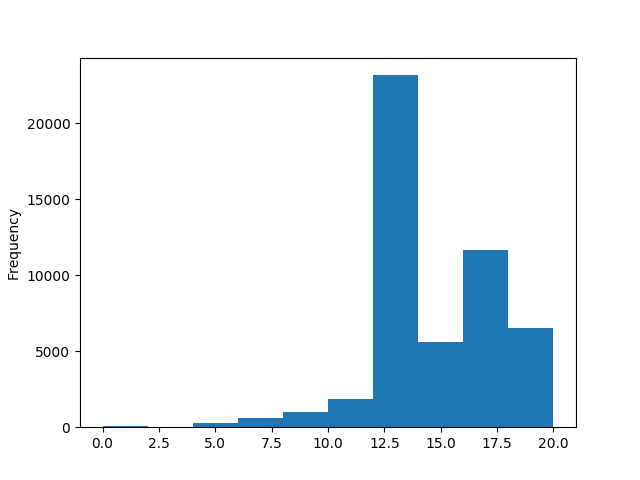
\includegraphics[scale=.8]{part_a}

\item

\begin{tabular}{ c c }
 Years & Observations \\
 \hline
 12 & 13896 \\ 
 16 & 11640 \\ 
 18 & 4670  \\ 
 20 & 1875 
\end{tabular}


\item

Below are the kernel density plots.

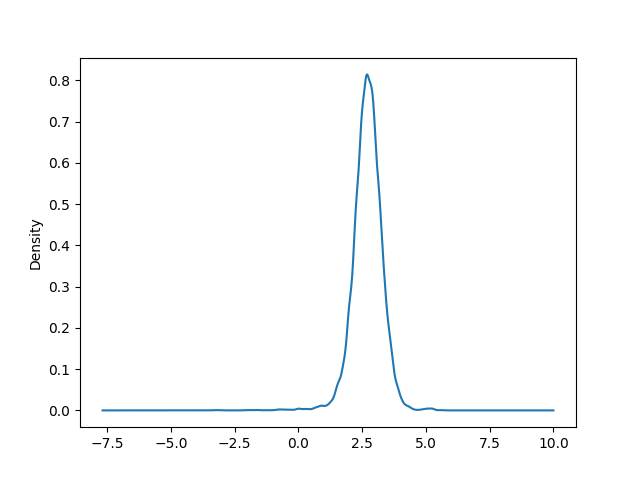
\includegraphics[scale=.8]{part_b_12}

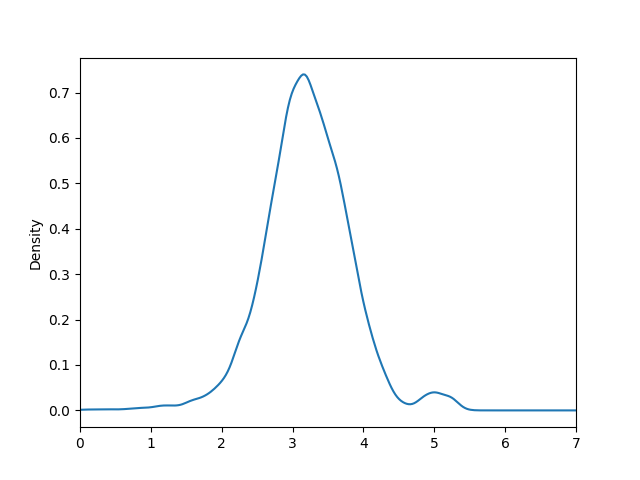
\includegraphics[scale=.8]{part_b_16}

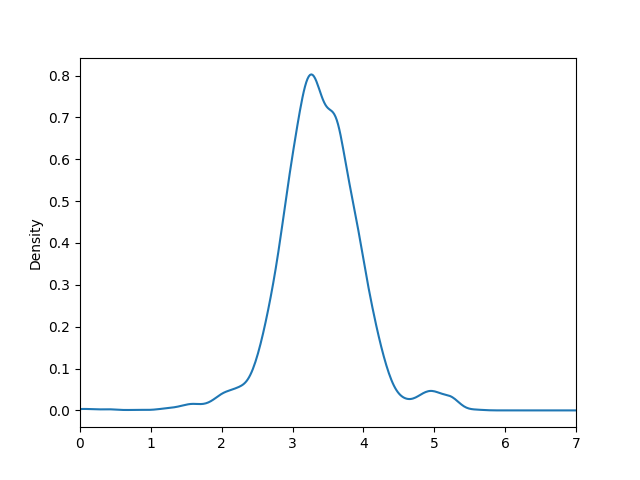
\includegraphics[scale=.8]{part_b_18}

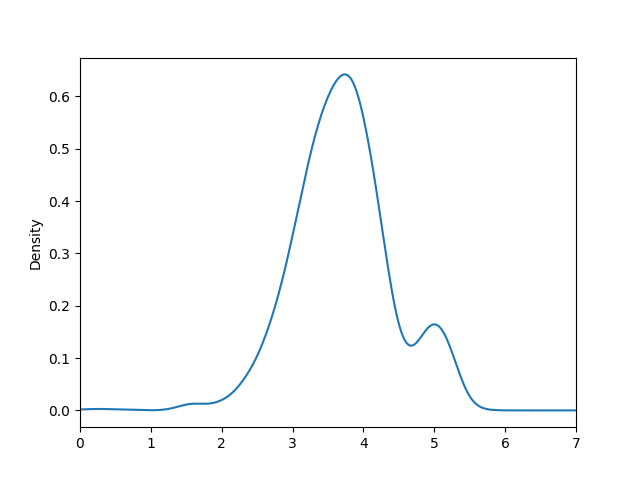
\includegraphics[scale=.8]{part_b_20}

\item The table below show the results.

\begin{tabular}{ c c c }
 Years & Mean & Variance \\
 \hline
 12 & 2.712 & 0.329 \\ 
 16 & 3.201 & 0.416 \\ 
 18 & 3.381 & 0.363 \\ 
 20 & 3.689 & 0.619    
\end{tabular}

By the table, we can see 20 years of education has the highest variance.


\item The table below show the results.

\begin{tabular}{ c c c c }
Year & 25th & 50th & 75th \\
\hline
12 & 2.403 & 2.733 & 3.055 \\
16 & 2.839 &	3.180 & 3.585 \\
18 & 3.062 &	3.362 & 3.710 \\
20 & 3.275 &	3.690 &	4.089 \\
\end{tabular}

\item The table below show the results.

\begin{tabular}{ c c }
Years & Difference \\
\hline
12 & 0 \\
16 & 0.489 \\
18 & 0.669 \\
20 & 0.977 \\
\end{tabular}

\item  The table below show the results.

\begin{tabular}{ c c c c c c } \\ Year 1 & Year 2 & Diff & SE & T-Value & Reject \\ 
 \hline 
12 & 12 & 0.0 & 0.00486691158299 & 0.0 & False \\ 
12 & 16 & -0.488918 & 0.00486691158299 & -100.457462777 & True \\ 
12 & 18 & -0.669176 & 0.00486691158299 & -137.494970241 & True \\ 
12 & 20 & -0.976912 & 0.00486691158299 & -200.725245359 & True \\ 
16 & 12 & 0.488918 & 0.00597543294539 & 81.821282852 & True \\ 
16 & 16 & 0.0 & 0.00597543294539 & 0.0 & False \\ 
16 & 18 & -0.180258 & 0.00597543294539 & -30.1665629463 & True \\ 
16 & 20 & -0.487994 & 0.00597543294539 & -81.6667908266 & True \\ 
18 & 12 & 0.669176 & 0.00882675326792 & 75.8122316274 & True \\ 
18 & 16 & 0.180258 & 0.00882675326792 & 20.4218095382 & True \\ 
18 & 18 & 0.0 & 0.00882675326792 & 0.0 & False \\ 
18 & 20 & -0.307736 & 0.00882675326792 & -34.8640263334 & True \\ 
20 & 12 & 0.976912 & 0.0181678405989 & 53.7714989472 & True \\ 
20 & 16 & 0.487994 & 0.0181678405989 & 26.8603431317 & True \\ 
20 & 18 & 0.307736 & 0.0181678405989 & 16.9385104793 & True \\ 
20 & 20 & 0.0 & 0.0181678405989 & 0.0 & False \\ 
\end{tabular}

\item The table below show the results.

\begin{center}
\begin{tabular}{lclc}
\toprule
\textbf{Dep. Variable:}    &      lwage       & \textbf{  R-squared:         } &     0.203   \\
\textbf{Model:}            &       OLS        & \textbf{  Adj. R-squared:    } &     0.203   \\
\textbf{Method:}           &  Least Squares   & \textbf{  F-statistic:       } &     2727.   \\
\textbf{Date:}             & Sat, 03 Feb 2018 & \textbf{  Prob (F-statistic):} &     0.00    \\
\textbf{Time:}             &     13:45:04     & \textbf{  Log-Likelihood:    } &   -30104.   \\
\textbf{No. Observations:} &       32081      & \textbf{  AIC:               } & 6.022e+04   \\
\textbf{Df Residuals:}     &       32077      & \textbf{  BIC:               } & 6.025e+04   \\
\textbf{Df Model:}         &           3      & \textbf{                     } &             \\
\bottomrule
\end{tabular}
\begin{tabular}{lcccccc}
                  & \textbf{coef} & \textbf{std err} & \textbf{t} & \textbf{P$>$$|$t$|$} & \textbf{[0.025} & \textbf{0.975]}  \\
\midrule
\textbf{const}    &       2.7121  &        0.005     &   516.939  &         0.000        &        2.702    &        2.722     \\
\textbf{educ\_16} &       0.4889  &        0.008     &    62.916  &         0.000        &        0.474    &        0.504     \\
\textbf{educ\_18} &       0.6692  &        0.010     &    63.969  &         0.000        &        0.649    &        0.690     \\
\textbf{educ\_20} &       0.9769  &        0.015     &    64.203  &         0.000        &        0.947    &        1.007     \\
\bottomrule
\end{tabular}
\begin{tabular}{lclc}
\textbf{Omnibus:}       & 10460.946 & \textbf{  Durbin-Watson:     } &     1.767   \\
\textbf{Prob(Omnibus):} &    0.000  & \textbf{  Jarque-Bera (JB):  } & 213631.163  \\
\textbf{Skew:}          &   -1.068  & \textbf{  Prob(JB):          } &      0.00   \\
\textbf{Kurtosis:}      &   15.460  & \textbf{  Cond. No.          } &      4.98   \\
\bottomrule
\end{tabular}
%\caption{OLS Regression Results}
\end{center}



\section{Python Code}

\begin{lstlisting}[language=Python]


\end{lstlisting}

\end{enumerate}



\end{document}